\begin{center}
\begin{figure}[bhtp]
    \centering
    \captionsetup{justification=centering, font=small, margin=0.5cm}
    \begin{subfigure}[b]{0.52\linewidth}
        \centering
        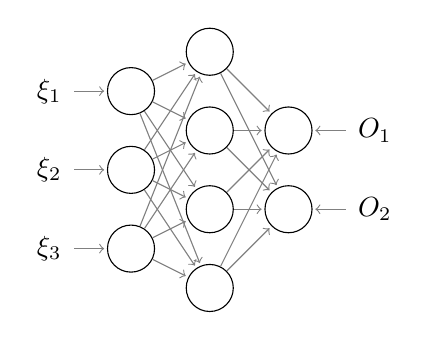
\begin{tikzpicture}[scale=1, shorten >=1pt,->,draw=black!50, node distance=1cm]
    \tikzstyle{every pin edge}=[<-,shorten <=1pt]
    \tikzstyle{neuron}=[circle,fill=black!25,minimum size=17pt,inner sep=0pt]
    \tikzstyle{input neuron}=[neuron, draw=black, fill=white!50];
    \tikzstyle{output neuron}=[neuron, draw=black, fill=white!50];
    \tikzstyle{hidden neuron}=[neuron, draw=black, fill=white!50];
    
    % Draw the input layer nodes
    \foreach \name / \y in {1,...,3}
    % This is the same as writing \foreach \name / \y in {1/1,2/2,3/3,4/4}
        \node[input neuron, pin=left:$\xi_{\y}$] (I-\name) at (0,-\y) {};

    % Draw the hidden layer nodes
    \foreach \name / \y in {1,...,4}
        \path[yshift=0.5cm]
            node[hidden neuron] (H-\name) at (1cm,-\y cm) {};
            
    % Draw the output layer node
    \node[output neuron, pin=right:$O_1$, right of=H-2] (O-1) {};
    \node[output neuron, pin=right:$O_2$, right of=H-3] (O-2) {};

    % Connect every node in the input layer with every node in the hidden layer.
    \foreach \source in {1,...,3}
        \foreach \dest in {1,...,4}
            \path (I-\source) edge (H-\dest);

    % Connect every node in the hidden layer with the output layer
    \foreach \source in {1,...,4}
        \foreach \dest in {1,...,2}
        \path (H-\source) edge (O-\dest);

\end{tikzpicture}
        \caption{Two-layer perceptron}
    \end{subfigure}
    \begin{subfigure}[b]{0.46\linewidth}
        \centering
        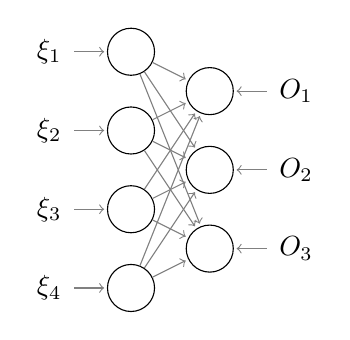
\begin{tikzpicture}[scale=1, shorten >=1pt,->,draw=black!50, node distance=1cm]
    \tikzstyle{every pin edge}=[<-,shorten <=1pt]
    \tikzstyle{neuron}=[circle,fill=black!25,minimum size=17pt,inner sep=0pt]
    \tikzstyle{input neuron}=[neuron, draw=black, fill=white!50];
    \tikzstyle{output neuron}=[neuron, draw=black, fill=white!50];
    
    % Draw the input layer nodes
    \foreach \name / \y in {1,...,4}
    % This is the same as writing \foreach \name / \y in {1/1,2/2,3/3,4/4}
        \node[input neuron, pin=left:$\xi_{\y}$] (I-\name) at (0,-\y) {};

    % Draw the hidden layer nodes
    \foreach \name / \y in {1,...,3}
        \path[yshift=-0.5cm]
            node[output neuron, pin=right:$O_\y$] (O-\name) at (1cm,-\y cm) {};
    
    % Connect every node in the input layer with every node in the hidden layer.
    \foreach \source in {1,...,4}
        \foreach \dest in {1,...,3}
            \path (I-\source) edge (O-\dest);
\end{tikzpicture}
        \caption{Simple perceptron}
    \end{subfigure}
    \caption{Examples of perceptrons}
    \label{fig:1}
\end{figure}
\end{center}